\chapter{Methodology}
\section{Retrieving the data}
I can access the active eBay listings near me by fetching data recursively from the eBay API. I wrote a small seeder script that stores the data in csv format and saves it locally. From there, I can easily read the csv in my notebook. The Foursquare data will be loaded within the code cells.
\section{Handling missing information and combining the two datasets}
After fetching the data, it is time to combine and unify the datasets, so I can work with coherent data in the next steps. For my purposes, it will be sufficient to have the following columns for both datasets:
\begin{itemize}
	\item Name of business/seller/store/item
	\item City
	\item State
	\item Latitude
	\item Longitude
	\item Source (eBay/Foursquare)
\end{itemize}
This is what the two datasets look like after fetching:
\begin{figure}[H]
	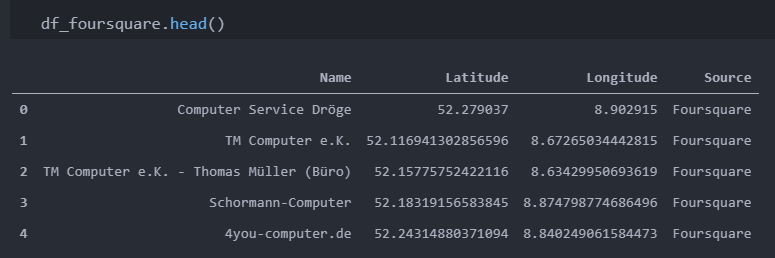
\includegraphics[width=\textwidth]{Bilder/Foursquare.PNG}
	\caption{Foursquare dataset right afer fetching with some columns already removed}
\end{figure}
\begin{figure}[H]
	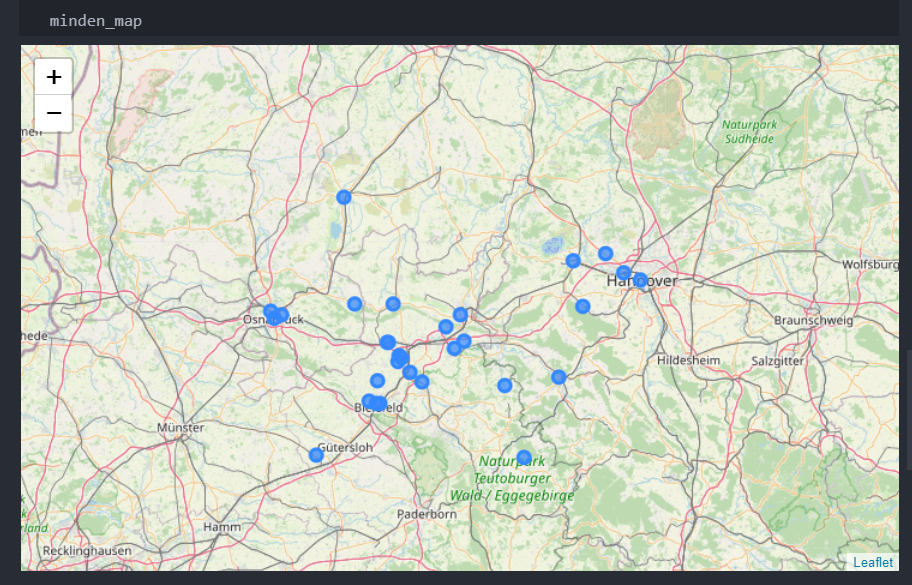
\includegraphics[width=\textwidth]{Bilder/Foursquare_Map.PNG}
	\caption{Foursquare dataset visualized in map}
\end{figure}
\begin{figure}[H]
	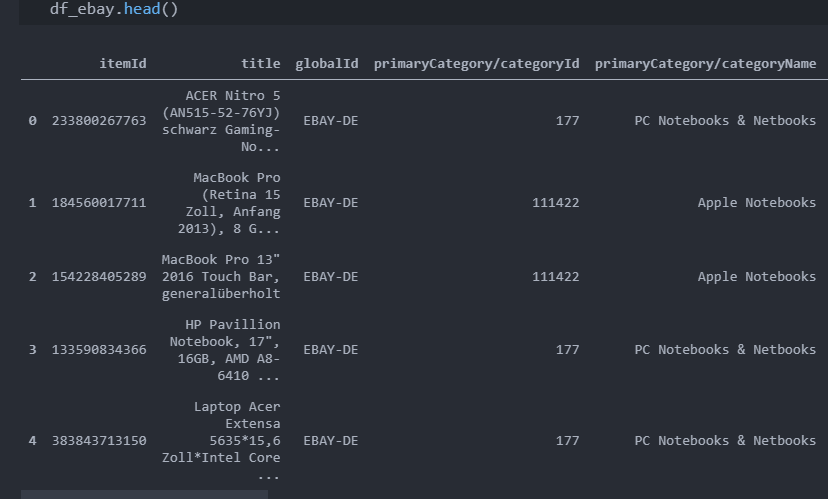
\includegraphics[width=\textwidth]{Bilder/eBay.PNG}
	\caption{Excerpt of eBay dataset right afer fetching}
\end{figure}

The Foursquare dataset is missing city and state, while the eBay dataset is missing coordinates unfortunately, as well as state. In the next step, I will preprocess the data and add the missing columns.

To preprocess the data, I will use OpenStreetMap\footnote{https://geocoder.readthedocs.io/providers/OpenStreetMap.html}. It provides a reverse geocoding function, allowing to search for locations for example by name or coordinates and receiving vast information in return. See below for the code and result.

\begin{figure}[H]
	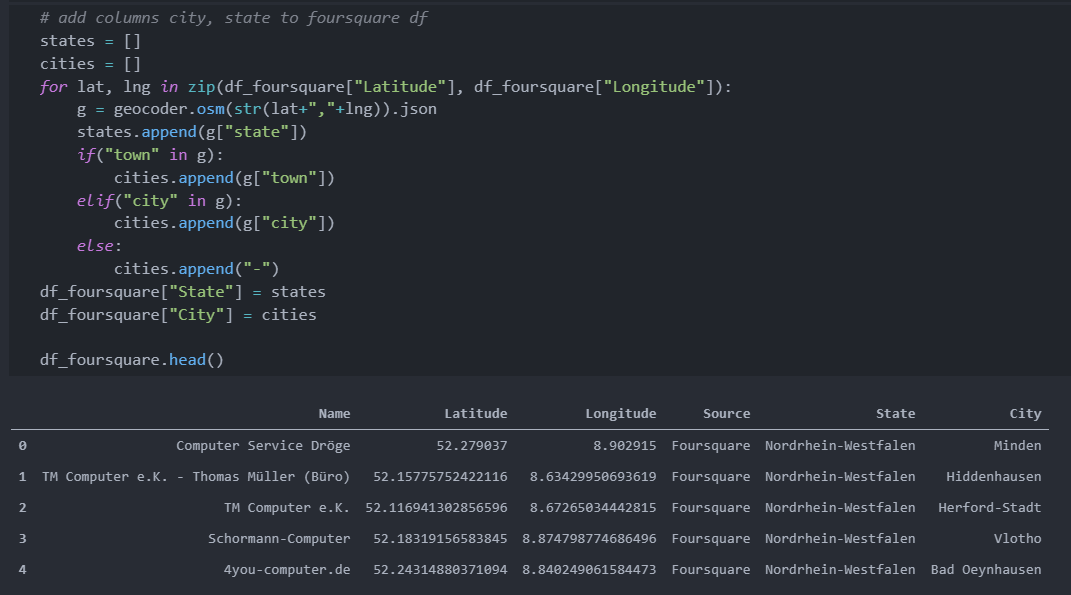
\includegraphics[width=\textwidth]{Bilder/Foursquare_preprocessed.PNG}
	\caption{Foursquare data with added state and city}
\end{figure}

The eBay data is missing state, latitude and longitude. These columns will also be added by using OpenStreetMap. See the following results.

\begin{figure}[H]
	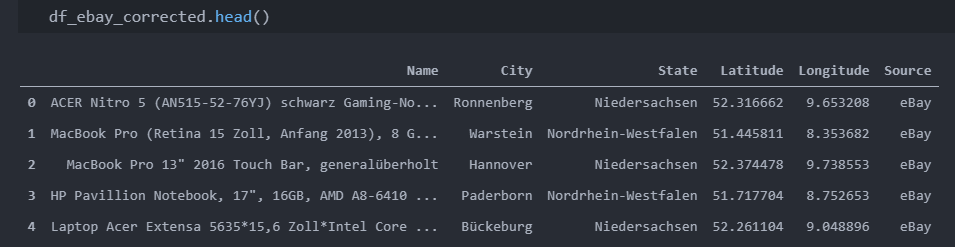
\includegraphics[width=\textwidth]{Bilder/eBay_preprocessed.PNG}
	\caption{eBay data with added state and coordinates}
\end{figure}
\begin{figure}[H]
	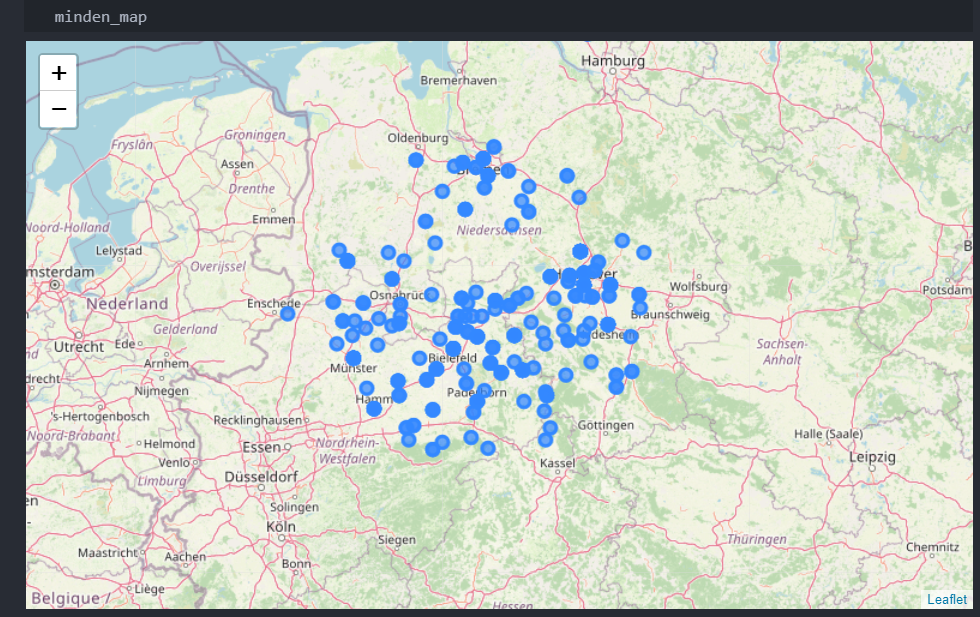
\includegraphics[width=\textwidth]{Bilder/eBay_Map.PNG}
	\caption{eBay dataset visualized in map}
\end{figure}

The two datasets are now combined and stored as a csv locally, to make sharing the data easier. This coherent structure now allows for some exploratory data analysis in the following subsections.
\section{Exploratory data analysis}
In this section, I will demonstrate how I managed to get a general overview over the data. This chapter only covers methodology, the results are discussed in \ref{results}.
\subsection{Statistical key figures and indicators}
To begin with some basic operations after creating a combined dataset, I described the given dataframe.
\begin{figure}[H]
	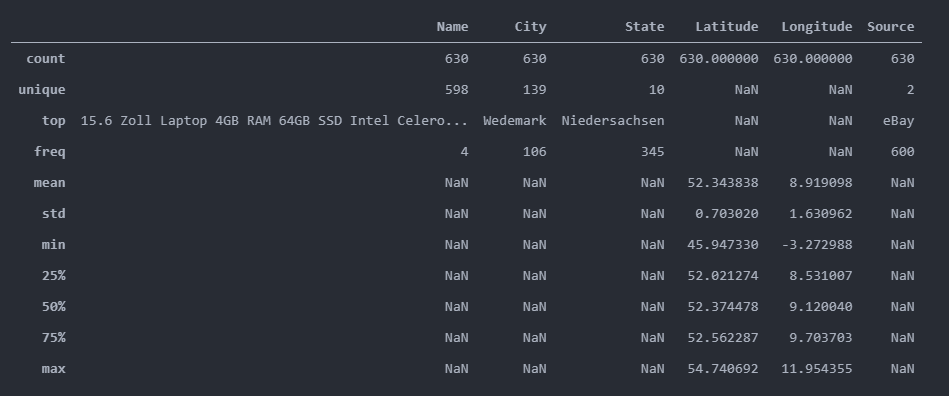
\includegraphics[width=\textwidth]{Bilder/general_findings.PNG}
	\caption{Description of dataset}
\end{figure}
\subsection{Visualizing entries using a map}
\begin{figure}[H]
	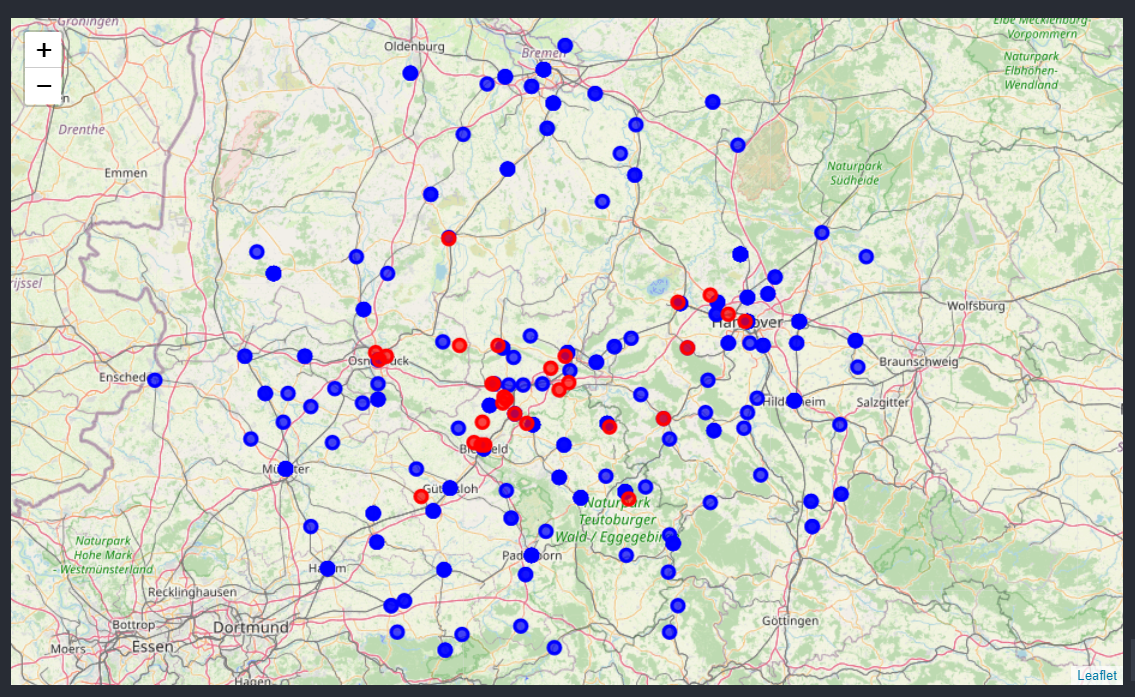
\includegraphics[width=\textwidth]{Bilder/combined_map.PNG}
	\caption{Visualization of dataset}
\end{figure}
This is what the map looks like when both sources are considered. Foursquare entries are colored red, eBay ones are blue.
\section{Machine learning}
Next, I will use the dataset to demonstrate the KNN algorithm. I want to cluster my entries by the state they are based in. KNN will be trained with the coordinates of the entries as independent variable. The target value therefore is the state of the entries.
\subsection{Clustering entries using KNN}
To set up KNN, the data first needs to be split by seperating independent and dependent variables.
\subsubsection{Display Columns}
To begin with and to get a feeling for the data I am working with, I chose to display the available columns within my dataset.
\begin{figure}[H]
	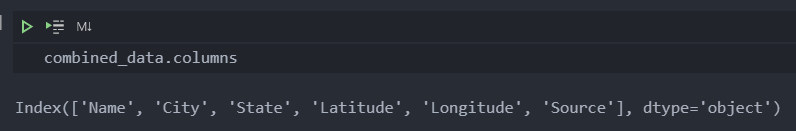
\includegraphics[width=\textwidth]{Bilder/display_columns.PNG}
	\caption{Columns of dataset}
\end{figure}
Because in my case, the state is dependent of the coordinates, the only three coordinates will be Latitude, Longitude and State. The first two being the independent variable, the latter being the target value that depends on the first two. So for the next step, choose X and y accordingly.
\subsubsection{Select columns for X and y}
As explained, X will contain Latitude and Longitude, whereas y will consist of the state.
\begin{figure}[H]
	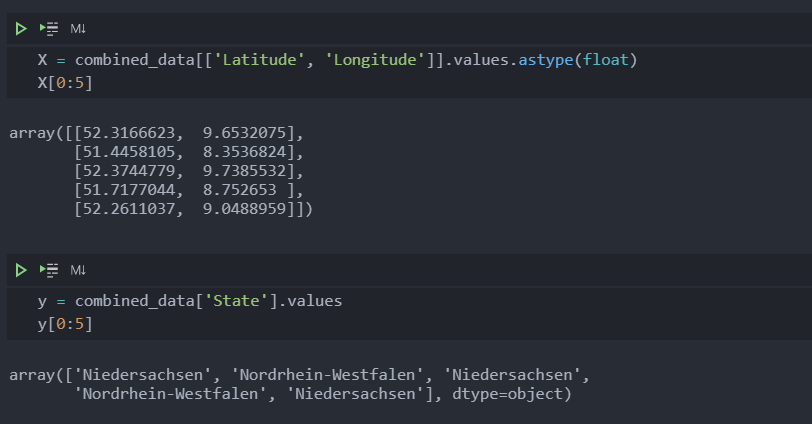
\includegraphics[width=\textwidth]{Bilder/select_columns.PNG}
	\caption{Selecting columns for KNN}
\end{figure}
Note that the coordinates are not standardized yet, and therefore need to be preprocessed. As of now, y also contains categorical data. The data will be hot encoded in the next step.
\subsubsection{Preprocess X and y}
Data Standardization give data zero mean and unit variance, it is good practice, especially for algorithms such as KNN which is based on distance of cases. Therefore, I begin with scaling X as in the course example.
\begin{figure}[H]
	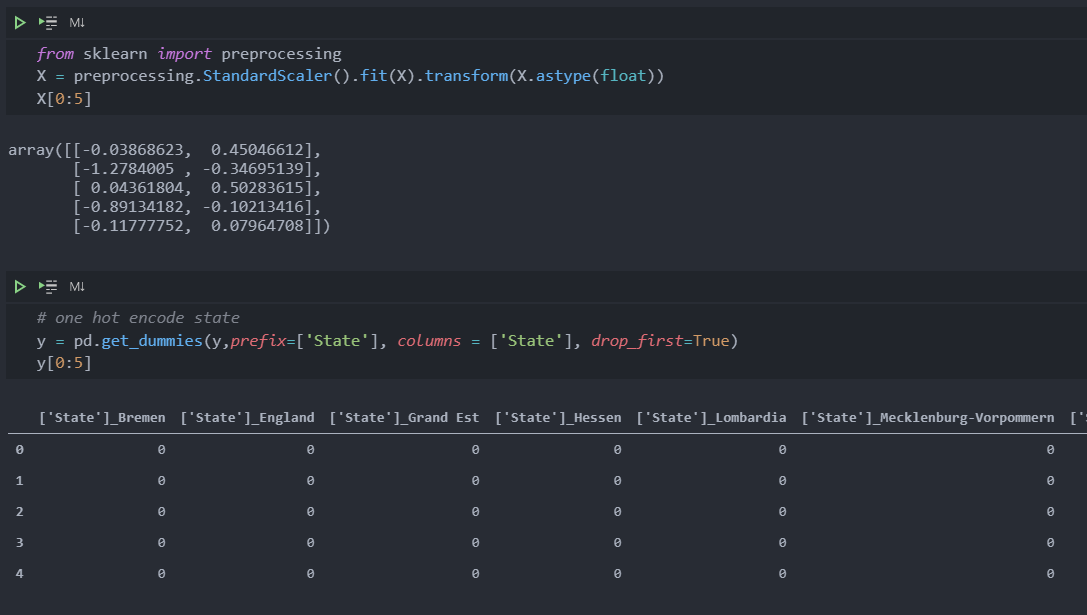
\includegraphics[width=\textwidth]{Bilder/preprocess_columns.PNG}
	\caption{Preprocessing X and y}
\end{figure}
Additionaly, I also one hot encoded the categorical state value. Note that there are states which are further away than 100km. This is because of the geocoder api and will be explained in chapter \ref{discussion}.
\subsubsection{Define test and train set}
Next, the data will be split into train and test set.
\begin{figure}[H]
	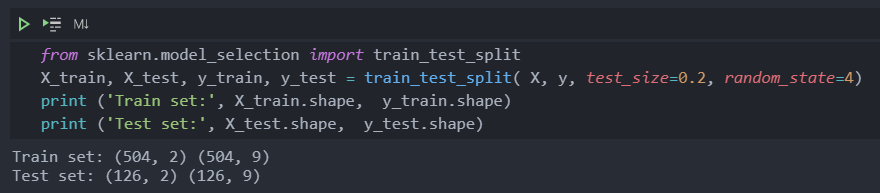
\includegraphics[width=\textwidth]{Bilder/define_test_train.PNG}
	\caption{Test Train Split}
\end{figure}
\subsubsection{Begin classification}
With the test and train set in hand, I can now find most accurate k for KNN. In the plot below, ks from 0 to 100 were tested.
\begin{figure}[H]
	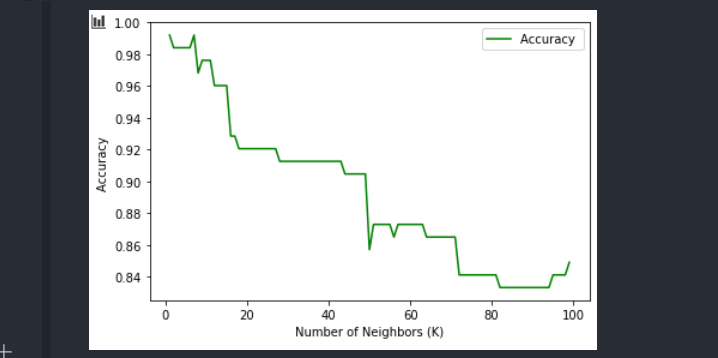
\includegraphics[width=\textwidth]{Bilder/finding_best_k.PNG}
	\caption{Finding best k for KNN}
\end{figure}
0 and 6 were the most accurate. I will continue using k=6 in the following steps when making the prediction and once again comparing the accuracy.
\begin{figure}[H]
	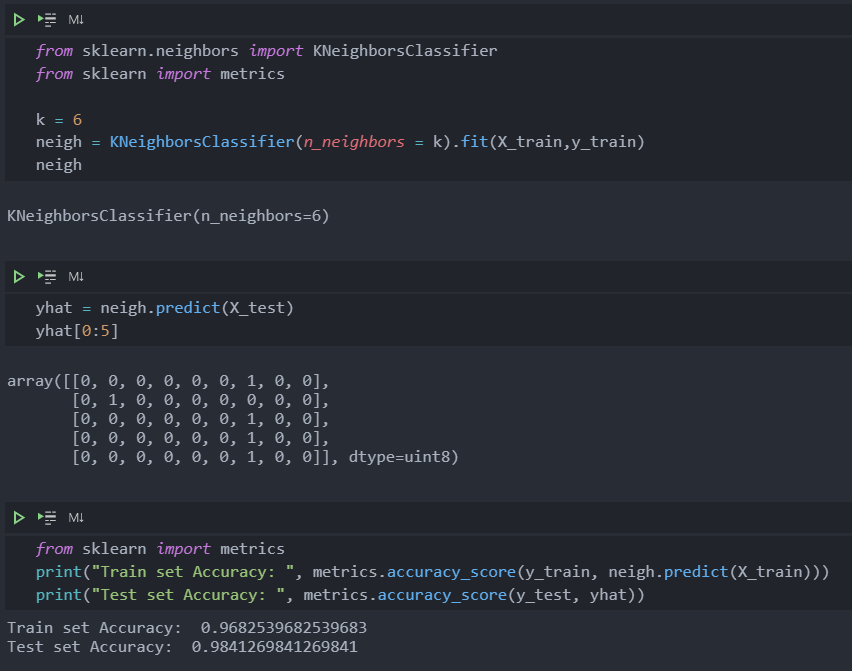
\includegraphics[width=\textwidth]{Bilder/predict_state.PNG}
	\caption{Predicting state based on coordinates and accuracy}
\end{figure}